%! Tex program = xelatex
\documentclass{article}

%\usepackage[UTF8]{ctex}
\usepackage{amsmath,amssymb}
\usepackage{ntheorem}
\usepackage[letterpaper,top=2cm,bottom=2cm,left=3cm,right=3cm,marginparwidth=1.75cm]{geometry}%table package
%Table
\usepackage{multirow,booktabs}
\usepackage{makecell}
%字体颜色
\usepackage{color}
\usepackage[dvipsnames]{xcolor}  % 更全的色系
%代码
\usepackage[OT1]{fontenc}
% MATLAB 代码风格
%\usepackage[framed,numbered,autolinebreaks,useliterate]{/Users/anye_zhenhaoyu/Desktop/Latex/mcode}
\usepackage{listings}
\usepackage{algorithm}
\usepackage{algorithmic}
%插图
\usepackage{graphicx}
%改变item格式
\usepackage{enumerate}
%物理
\usepackage{physics}
%extra arrows
\usepackage{extarrows}
% caption(居中指令)
%\usepackage[justification=centering]{caption}
\usepackage{caption}
% htpb
\usepackage{stfloats}
% pdf 拼接
\usepackage{pdfpages}
% 超链接url
\usepackage{url}

\def\RR{\mathbb{R}}
\def\ZZ{\mathbb{Z}}
\def\EE{\mathbb{E}}

\def\Trsp#1{#1^{\mathcal{T}}}

\def\bw{\boldsymbol{\omega}}
\def\ba{\boldsymbol{a}}
\def\bb{\boldsymbol{b}}
\def\bc{\boldsymbol{c}}
\def\bd{\boldsymbol{d}}
\def\bt{\boldsymbol{t}}
\def\bx{\boldsymbol{x}}
\def\by{\boldsymbol{y}}
\def\bz{\boldsymbol{z}}

\def\bA{\boldsymbol{A}}
\def\bB{\boldsymbol{B}}
\def\bC{\boldsymbol{C}}
\def\bE{\boldsymbol{E}}
\def\bO{\boldsymbol{O}}
\def\bX{\boldsymbol{X}}
\def\bY{\boldsymbol{Y}}

\def\Esolve{\textcolor{blue}{Solve: }}
\def\Eproof{\textcolor{blue}{Proof: }}

\def\suminf#1{\sum_{#1=-\infty}^{+\infty}}

\newtheorem{lemma}{Lemma}
\newtheorem{proof}{Proof}
\newtheorem*{theorem}{Theorem}

\graphicspath{{figures/}}


\begin{document}
\title{Homework 8}
\author{Zhen}
\maketitle


\section*{Problem 1}

\begin{enumerate}[(a)]
	\item 
		\textcolor{blue}{The output is:}\\
		\texttt{
			Newton's method\\
				number of iterations: 5\\
				solution: [-3.46573590e-01 -1.41533671e-10]\\
				value: 2.5592666966582156
			}

			\begin{figure}[H]
				\centering
				\begin{minipage}[b]{0.46\linewidth}
					\includegraphics[width=\linewidth]
					{/p1a/nt_traces.pdf}
					\caption{the trajectory of $\bx_k$}
				\end{minipage}
				\begin{minipage}[b]{0.46\linewidth}
					\includegraphics[width=\linewidth]
					{/p1a/nt_gap.pdf}
					\caption{the gap $f(\bx_k) - f(\bx^*)$}
				\end{minipage}
			\end{figure}
	\item
		\textcolor{blue}{The output is:}\\
		\texttt{
			Newton's method\\
				number of iterations: 8\\
				solution: [-3.46573573e-01  1.13424622e-08]\\
				value: 2.559266696658217
			}

			\begin{figure}[H]
				\centering
				\begin{minipage}[b]{0.46\linewidth}
					\includegraphics[width=\linewidth]
					{/p1b/nt_traces.pdf}
					\caption{the trajectory of $\bx_k$}
				\end{minipage}
				\begin{minipage}[b]{0.46\linewidth}
					\includegraphics[width=\linewidth]
					{/p1b/nt_gap.pdf}
					\caption{the gap $f(\bx_k) - f(\bx^*)$}
				\end{minipage}
			\end{figure}

\end{enumerate}

\newpage
\section*{Problem 2}
$$
\nabla f(\bw)=
-\sum_{i=1}^m\qty[1-\sigma(y_i\Trsp{\bx_i}\bw)]y_i\bx_i
$$


\begin{enumerate}[(a)]
	\item 
		$$
		\begin{aligned}
			\nabla^2f(\bw) = 
			&=-\sum_{i=1}^m
			\nabla\qty{\qty[1-\sigma(y_i\Trsp{\bx_i}\bw)]y_i\bx_i}
			\\&=
			-\sum_{i=1}^m
			-y_i^2\sigma'(y_i\Trsp{\bx_i}\bw)\bx_i\Trsp{\bx_i}
			\\&=
			\sum_{i=1}^m
			\sigma'(y_i\Trsp{\bx_i}\bw)\bx_i\Trsp{\bx_i}
		\end{aligned}
		$$
	
	\item
		\textcolor{blue}{The output is:}\\
		\texttt{
			Damped Newton's method\\
			number of iterations in outer loop: 20\\
			total number of iterations in inner loop: 10\\
			solution: [-1.47021646  4.44403104 -4.37591078]\\
			value: 2.8766810999687493
			}
		\begin{figure}[H]
			\centering
			\begin{minipage}[b]{0.46\linewidth}
				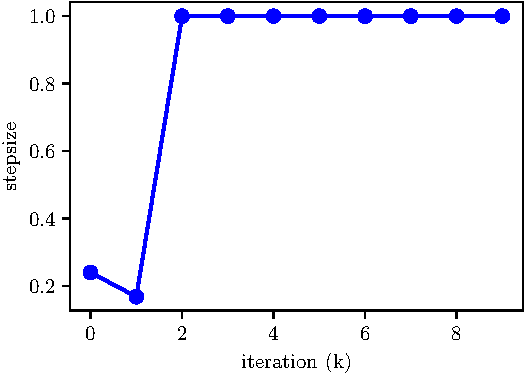
\includegraphics[width=\linewidth]
				{/p2b/p2bdnt_ss.pdf}
				\caption{the step sizes $t_k$}
			\end{minipage}
			\begin{minipage}[b]{0.46\linewidth}
				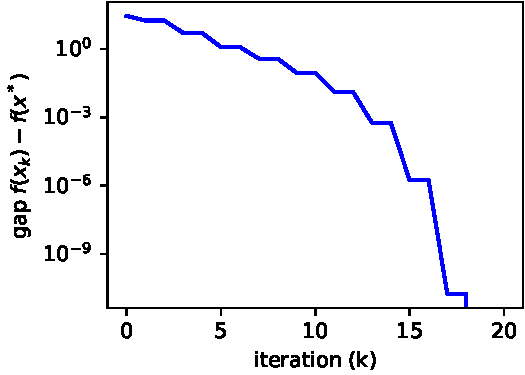
\includegraphics[width=\linewidth]
				{/p2b/p2bdnt_gap.pdf}
				\caption{the gap $f(\bx_k) - f(\bx^*)$}
			\end{minipage}
		\end{figure}
	\item
		It will cause a ``gradient ascent'':
		$$
		\Trsp{\mqty[1 & 1 & 0]}\rightarrow\Trsp{\mqty[-28.5 & -4.8 & 44.9]}\rightarrow\Trsp{\mqty[34330.7 & 5659.0 & -54500.0]}\rightarrow\cdots
		$$
\end{enumerate}

\section*{Problem 3}
\begin{enumerate}[(a)]
	\item By the fact that $f'(x)=4(x-a)^3$, $f''(x)=12(x-a)^2$, 
		$$
		\Delta x = 
		\frac{f'(x)}{f''(x)}=\frac{1}{3}(x-a)
		$$
	\item
		$$
		\begin{aligned}
			&
			x_{k+1}=x_k-\frac{1}{3}(x_k-a)
			\\ \Longrightarrow\ &
			x_{k+1}-a=\frac{2}{3}(x_k-a)
			\\ \Longrightarrow\ &
			y_{k+1}=\frac{2}{3}y_k
		\end{aligned}
		$$
	\item
		When $k\to0$,
		$$
		\abs{x_k-a}=\qty(\frac{2}{3})^k\abs{x_0-a}=\exp[-\ln(\frac{3}{2})k]\abs{x_0-a}\longrightarrow 0
		$$
\end{enumerate}

\section*{Problem 4}

\begin{enumerate}[(a)]
	\item 
		\textcolor{blue}{The output is:}\\
		\texttt{
			lambda =  2\\
			number of iterations: 169\\
			solution: [1.00000000e+00 9.24600449e-09]\\
			value: 6.5
			}
		\begin{figure}[H]
			\centering
			\begin{minipage}[b]{0.46\linewidth}
				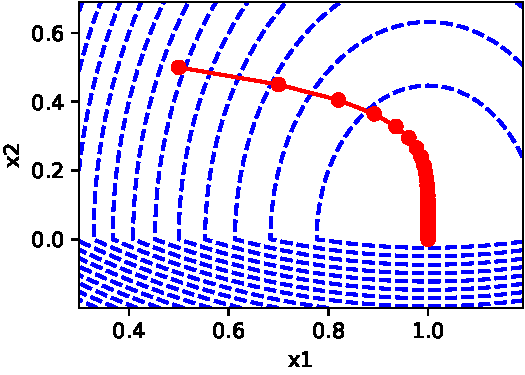
\includegraphics[width=\linewidth]
				{/p4/ista_traces_lambda2.pdf}
				\caption{the trajectory of $\bx_k$}
			\end{minipage}
			\begin{minipage}[b]{0.46\linewidth}
				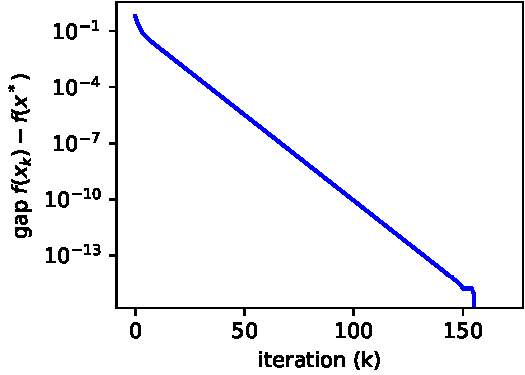
\includegraphics[width=\linewidth]
				{/p4/ista_gap_lambda2.pdf}
				\caption{the gap $f(\bx_k) - f(\bx^*)$}
			\end{minipage}
		\end{figure}
	\item 
		\textcolor{blue}{The output is:}\\
		\texttt{
			lambda =  1\\
			number of iterations: 169\\
			solution: [1.25       0.99999999]\\
			value: 4.875
			}
		\begin{figure}[H]
			\centering
			\begin{minipage}[b]{0.46\linewidth}
				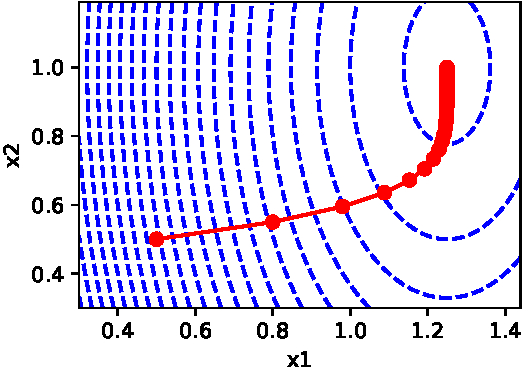
\includegraphics[width=\linewidth]
				{/p4/ista_traces_lambda1.pdf}
				\caption{the trajectory of $\bx_k$}
			\end{minipage}
			\begin{minipage}[b]{0.46\linewidth}
				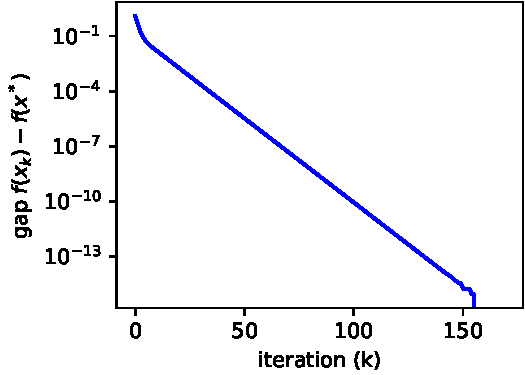
\includegraphics[width=\linewidth]
				{/p4/ista_gap_lambda1.pdf}
				\caption{the gap $f(\bx_k) - f(\bx^*)$}
			\end{minipage}
		\end{figure}
		\textcolor{blue}{\textbf{No zero in $\bw^*$.}}
	\item 
		\textcolor{blue}{The output is:}\\
		\texttt{
			lambda =  6\\
			number of iterations: 38\\
			solution: [ 1.85659632e-09 -0.00000000e+00]\\
			value: 8.500000000000002
			}
		\begin{figure}[H]
			\centering
			\begin{minipage}[b]{0.46\linewidth}
				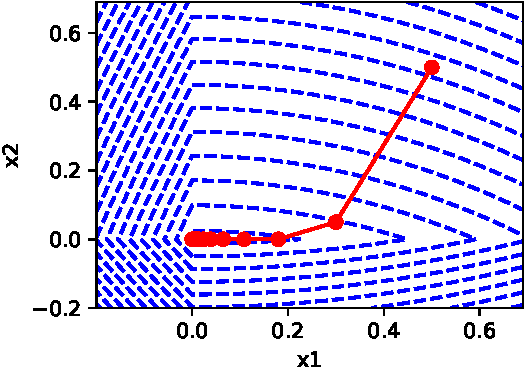
\includegraphics[width=\linewidth]
				{/p4/ista_traces_lambda6.pdf}
				\caption{the trajectory of $\bx_k$}
			\end{minipage}
			\begin{minipage}[b]{0.46\linewidth}
				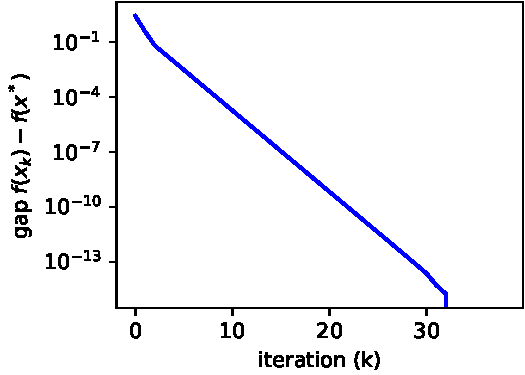
\includegraphics[width=\linewidth]
				{/p4/ista_gap_lambda6.pdf}
				\caption{the gap $f(\bx_k) - f(\bx^*)$}
			\end{minipage}
		\end{figure}
		\textcolor{blue}{\textbf{There are 2 zeros in $\bw^*$.}}
\end{enumerate}


\end{document}

